\chapter{Future Work Plan}
\label{chap:future}

In this chapter we briefly discuss how we plan to approach the aim, objectives and research questions as stated in Chapter \ref{chap:aimsObj}. We give a broad overview in terms of the years of the PhD, the planned papers treating the objectives and research questions. Further we present important milestones, relevant conferences and a Gantt-Chart reflecting all the details \ref{fig:gantt}.

TODO: IMPORTANT is to note that the benefits do NOT come from my library but from the usage of the pure functional paradigm. the library just puts it into a more convenient form. So the library is again just a tool which allows us to research how far we can get in robustness, verification and correctness in ABS when pure functional programming as compared to the approach of object-oriented Java in the form of Repast.

\section{Overall Approach}

\subsection{Aim}
First a library for general-purpose ABS in Haskell is built which serves as the primary object to study the benefits and drawbacks. \footnote{Note that - despite it takes quite some effort - this library in itself is no the contribution of this Ph.D. but just a means to an end which allows to research and investigate the objectives and research questions and substantiate the hypotheses.}

To explore the further potential of formal reasoning and verification in functional ABS on the example of Sugarscape requires the implementation of Sugarscape in the Haskell ABS library and to replicate and align the dynamics with the one given in the original model. Apply reasoning to the bilateral decentralized bartering process in the Sugarscape model and find out how far reasoning can be utilized and to what extent one can reason about e.g. equilibrium and dynamics in a pure functional ABS and if it is possible at all.

TODO:
- Why ACE and Social Simulation? Did i only pick these fields because they are easily applicable to the problems I want to solve? Which properties do they exhibit which make them interesting for my problem? Just to say that "Sugarscape and bilateral decentralized bartering is interesting and fascinates me" is not enough in a final viva/thesis/paper.	

TODO:
instead of writing a paper on every bit of research conducted we will write a report on the following studies which need to be conducted:

\begin{itemize}
	\item Comparing the pure functional and object oriented paradigm to implement ABS
	\item Comparing Repast Java and Functional Reactive ABS
	\item Replicating \& aligning Sugarscape in FrABS 
\end{itemize}

Out of these reports then papers can be condensed as required. We do not yet know exactly which papers we will write but we plan for up to 3 papers targeted as journal papers.

\begin{enumerate}
	\item Towards pure functional programming in ABS - introduces the new approach, reports benefits and drawbacks and shows examples.
	\item Levels of Correctness of Agent-Based Simulations - introduces the real power of the FrABS approach: ability to reason about ABS, specification-testing using QuickCheck, guaranteed absence of bugs,... to show how far we can go in asserting the correctness of an ABS (the hypothesis: further than in approaches so far)
\end{enumerate}

\subsection{Objectives}


\section{Years Overview}

\subsection{1st Year: foundations - building the tool}
In the first year, all was about orientation, prototyping, experimenting and finding out what the PhD is \textit{really} going to be about. Foundational work was layed out, which in the paper on update-strategies and the ommited part on programming paradigms. By now we have a properly working prototype of the library with a few good, diverse examples of implemented ABS including SugarScape and Agent\_Zero. At this point we have gathered enough information, experience and the library is sufficiently advanced to know that Haskell is definitely not a dead end.

\subsection{2nd Year: Shaping the new approach - comparing the tool}
In the 2nd year the aim is to scientifically show the benefits and drawbacks of using Haskell implementing ABS in comparison to the existing technologies in the field like Repast and plain Java. The goal is to write two papers, one which treats general questions in how Haskell can be used in ABS and its potential benefits and drawbacks. The other paper will describe the novel approach, called functional reactive ABS, implemented in the library. 

\subsection{3rd Year: Selling the new approach - new methods through the tool}
ITS ALL ABOUT CORRECTNESS (this is probaly the only thing that FrABS really shines)

In the final year we want to focus on how Haskells unique reasoning abilities can be made of use in the field of ABS by looking into reasoning about the bilateral decentralized bartering process as it occurs in the Sugarscape model.
The remainder of the year is to focus on cleaning up the research and writing the final thesis. The plan is to start the writing of the final thesis around April 2019 with a 5-months writing-window and to submit on-time at end of September 2019.

\section{Planned Papers}
For the remainder of the PhD we planned for three papers where the first one is targeted as a research-paper with no intention of publishing and the other two papers to be targeted as journal papers.

\subsection{Towards pure functional programming in ABS Part I: Suitability of Haskell}

\subsection{Towards pure functional programming in ABS Part II: Functional Reactive ABS}
-> this paper looks into the specifics of the hybrid approach of FrABS: how time can be used. It asks if time can be turned back e.g. that time-travel may become possible. This facility would pose interesting new mechanisms for investigating the dynamics of Agent-Based Simulations: halting time, fast-forward and fast-backward. The backward-going is a novelty. Could we inject new random-seeds during execution? 

-> also it contains first hint at reasoning possibilities about the simple SIR model
		-> my emulation of SD using ABS is really an implementation of the SD model and follows it - they are equivalent
		-> my ABS implementation is the same as / equivalent to the SD emulation
			=> thus if i can show that my SD emulation is equlas to the SD model
			=> AND that the ABS implementation is the same as the SD emulation
			=> THEN the ABS implementation is an SD implementation, and we have shown this in code for the first time in ABS

\subsection{Will it Equilibrate? Reasoning about dynamics in ABS}
In this paper we will discuss the verification method we have developed using our FrABS implementation and QuickCheck. We describe the decentralized bilateral bartering process of the Sugarscape model and verify it.
-> purely reasoning about the bilateral trading in sugarscape.
	-> explain bilateral decentralized bartering
	-> general equilibrium theory
	-> give reason in code for the failure of reaching equilibrium

-> can we reason about the equilibrium prices in an ABS setting? e.g. show formally why equilibrium prices are not reached, under which circumstance they are reached,...
			-> need to combine General Equilibrium Theory
			-> with Bilateral decentralized exchange
			-> with Agent-Based Simulation 
			
\section{Conferences}
\begin{itemize}
	\item \textbf{Multi-Agent Systems AAMS} - General Multi-Agent Systems and Agent-Based Modelling \& Simulation, Deadline in November
	\item \textbf{Social Simulation Conference SSC} - New Methods and models in simulation, Deadline in March
	\item \textbf{Symposium on Trends in Functional Programming} - Functional programming stuff, Deadline in May
\end{itemize}

\section{Mile-Stones}
\begin{itemize}
	\item 2017 31st March - finished and submit Paper 
	\item 2017 18th June - Finished writing 1st year report 
	\item 2017 21st July - 1st Annual Review
	\item 2017 October - 2nd year starts
	\item 2018 May - Submit Paper on FrABS
	\item 2018 October - 3rd year starts
	\item 2019 February - Submit Paper on Verification
	\item 2019 April - Begin of thesis-writing
	\item 2019 September - Submit Thesis
	\item 2019 30th September - official end of PhD
	\item 2020 30th September - end of pending-period
\end{itemize}

\label{app:gantt}
\begin{landscape}
	\begin{figure}
		\label{fig:gantt}
  		\caption{Gantt-Chart for remaining PhD}
  		\centering
  		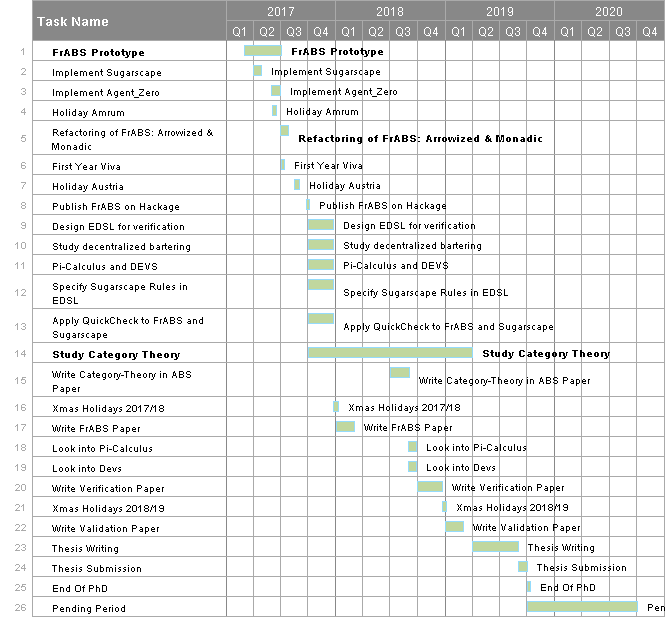
\includegraphics[width=1.2\textwidth]{./charts/gantt.png}
	\end{figure}
\end{landscape}